\section{\secfunctions}
\label{sec_functions}

In this section, we introduce the formal definition of a function, look at examples of functions defined by formulas, and discuss how to visually represent functions.  The definition of a function requires sets, so we begin with the names of some common infinite sets of numbers.

%%%%%%%%%%%%%%%%%%%%%%%%%%%%%%%%%%
\newcommand{\subinfsetsnumbers}{Infinite sets of numbers}
\subsection{\subinfsetsnumbers}
\label{sub_infinite_sets_numbers}

The definition of a function involves sets. Functions in discrete contexts often involve sets of integers, natural numbers, or rational numbers as defined in \Cref{defn_integers} and \Cref{defn_fraction_rational}. It is convenient to have names for such sets.

\begin{defn}[Sets of integers]
\label{defn_sets_of_integers}  
~
    \begin{apart}
        \item The \vocab{set of all integers}\footnote{Why is $Z$ is used for the set of integers? Part of the reason is because $I$ already stands for many other things in mathematics and physics. But why $Z$?  In the past, a lot of European mathematics was written in German and the German word for numbers is \emph{Zahlen} which starts with the letter $Z$.  The name $Z$ for the set of all integers was introduced by the German mathematician David Hilbert who is rightfully famous for many other reasons.  Source: Integer. (2024, May 20). In \emph{Wikipedia}. \url{https://en.wikipedia.org/wiki/Integer}.} 
        is $$\mathbb{Z} = \{ \ldots, -3,-2,-1,0,1,2,3,\ldots\}.$$   

        \item The \vocab{set of all positive integers} is $$\mathbb{Z}^+=\{1,2,3,\ldots\}.$$
        
        \item The \vocab{set of all natural numbers} (or \vocab{set of all non-negative integers}) is
        $$\mathbb{N} = \{0, 1,2,3,\ldots\}.$$
    \end{apart}
\end{defn}

Let's look at an example involving these sets.

\begin{exam}[Sets of integers]
\label{exam_sets_integers}
~
    \begin{apart}
        \item Which of the sets $\mathbb{Z}$, $\mathbb{Z}^+$, and $\mathbb{N}$ have the integer 0 as an element?
            \begin{soln}
                The integer 0 is an element of $\mathbb{Z}$ and $\mathbb{N}$, but it is not an element of $\mathbb{Z}^+$.
            \end{soln}

        \item Which of the sets $\mathbb{Z}$, $\mathbb{Z}^+$, and $\mathbb{N}$ are subsets of the others?
            \begin{soln}
                Every positive integer is a natural number so $\mathbb{Z}^+$ is a subset of $\mathbb{N}$.  Every positive integer and every natural number is an integer so $\mathbb{Z^+}$ and $\mathbb{N}$ are subsets of $\mathbb{Z}$.  And, of course, each set is a subset of itself too.
            \end{soln}
        
    \end{apart}
\end{exam}

Functions in more continuous contexts, like algebra or calculus, often involve real numbers.  A formal definition of real numbers requires mathematics beyond this textbook, but we start with a casual form of the definition.

\begin{defn} [Real numbers]
\label{defn_reals}
~
    \begin{apart}
        \item A \vocab{real number} is any number that can be represented in decimal notation. For example, each of the following numbers is a real number:  523.7, $34 = 34.0$, $\frac{3}{8} = .375$, $-\sqrt{2} = -1.414213\ldots$, and $\pi = 3.141592\ldots$. The \ldots indicates that the decimal representation continues.
        \item When the decimal notation for a real number repeats forever, we use \vocab{bar} notation. For example, $$\frac{7}{11} = 0.636363\ldots = 0.\overline{63}.$$
    \end{apart}
\end{defn}

It is useful to have a notation for commonly used sets of real numbers.

\begin{defn}[Sets of real numbers]
\label{defn_sets_of_real_numbers}  
~
    \begin{apart}
        \item The \vocab{set of all rational numbers}\footnote{The letter $Q$ comes from the word ``quotient''.} is 
        denoted $\mathbb{Q}$.  For example, $\frac{3}{8}$, $^-\frac{7}{11} = \frac{-7}{11}$, and $34 = \frac{34}{1}$ are elements of $\mathbb{Q}$.
       
        \item The \vocab{set of all real numbers} is denoted
        $\mathbb{R}.$  For example, each of the following real numbers is an element of $\mathbb{R}$: 523.7, $34$, $\frac{3}{8}$, $^-\frac{7}{11}$, $-\sqrt{2}$, and $\pi$.
        
        \item If $S$ is a subset of real numbers, then the set $S^+$ is the set of all positive numbers in $S$ and the set $S^*$ is the set of all nonzero numbers in $S$.  For example, 
        $$\mathbb{R}^+ = \text{set of all positive real numbers}$$
        and  $$\mathbb{R}^* = \text{set of all nonzero real numbers}.$$       
    \end{apart}
\end{defn}

Let's look at an example.

\begin{exam}[Sets of real numbers]
\label{exam_sets_reals}
~
    \begin{apart}
        \item Which of the sets $\mathbb{Q}$, $\mathbb{R}$, $\mathbb{R}^+$, and $\mathbb{R}^*$ have the integer 0 as an element?
            \begin{soln}
                The integer 0 can be written as a fraction, for example $0 = \frac{0}{1}$.  Thus 0 is an element of $\mathbb{Q}$.  The integer 0 can be written as 0.0 (or just 0).  Thus 0 is an element of $\mathbb{R}$.  Since the integer 0 is not positive, 0 is not an element of $\mathbb{R}^+$.  Since the integer 0 is not nonzero, 0 is not an element of $\mathbb{R}^*$.
            \end{soln}
        \item Which of the sets $\mathbb{Z}$, $\mathbb{Q}$, and $\mathbb{R}$ are subsets of the others?
            \begin{soln}
                Any integer $n$ can be written as a fraction, for example $n = \frac{n}{1}$.  Thus $n$ is an element of $\mathbb{Q}$ and so $\mathbb{Z}$ is a subset of $\mathbb{Q}$.  Any integer $n$ can also be written as a real number, for example $n = n.0$ (or just $n$).  Thus $n$ is an element of $\mathbb{R}$ and so $\mathbb{Z}$ is a subset of $\mathbb{R}$.  Any rational number $\frac{a}{b}$, where $a$ is an integer and $b$ is a nonzero integer, can be written as a decimal by dividing $a \div b$.  We might get a terminating decimal, like $\frac{3}{8}=0.375$, or we might get a repeating decimal, like $\frac{7}{11} = 0.636363\ldots = 0.\overline{63}$.  (It turns out we cannot get a non-repeating decimal.)  Thus $\frac{a}{b}$ is an element of $\mathbb{R}$ and so $\mathbb{Q}$ is a subset of $\mathbb{R}$.
            \end{soln}
    \end{apart}
\end{exam}

There is a special notation for subsets of real numbers that are defined by inequalities.

\begin{defn}[Intervals]
\label{defn_intervals} 
~
    \begin{apart}
        \item An \vocab{interval} is a set of all real numbers $x$ between two real numbers known as \vocab{bounds}. For example, the set of all real numbers $x$ such that $11 \le x < 12$ is an interval bounded below by 11 and bounded above by 12. The integer 11 is an element of the interval, but the integer 12 is not an element of the interval.
        \item An \vocab{unbounded interval} (or \vocab{ray}) is a set of all real numbers greater than a real number or a set of all real numbers less than a real number.  For example, the set of all real numbers $x$ such that $x\ge 4.32$ is an unbounded interval. The real number 4.32 is an element of that interval. The set of negative real numbers $x$ is the unbounded interval defined by  $x<0$.  The real number 0 is not an element of that interval.
        \item We can abbreviate an interval using \vocab{interval notation} where a square bracket indicates that the bound is included, whereas a round bracket indicates that the bound is excluded.  When the interval is unbounded, we use $\infty$ to indicate that the interval has no upper bound and $-\infty$ to indicate that the interval has no lower bound.  For example, the interval described by the inequality $11 \le x < 12$ is denoted $[11,12)$ and the positive real numbers is denoted $(0,\infty)$.
        Occasionally we write the full set of real numbers $\mathbb{R}$ as the interval $(-\infty,\infty).$  \Cref{table_interval_notation} shows examples of each type of interval notation.

        \begin{table}[ht]
            \centering
            \begin{tabular}{l | c|c|c|c}
                Interval 
                & $a \le x \le b$ 
                & $a \le x < b$
                & $a < x \le b$
                & $a < x < b$           \\ \hline
                Notation 
                & $[a,b]$ 
                & $[a,b)$
                & $(a,b]$
                & $(a,b)$
            \end{tabular}
            
            \vspace{.15in}
            % Space between lines of table
            
            \begin{tabular}{l | c|c|c|c | c}
                Unbounded Interval 
                & $x \ge a$
                & $x > a$
                & $x \le b$
                & $x < b$
                & $x$
                \\ \hline  
                Notation 
                & $[a,\infty)$
                & $(a,\infty)$
                & $(-\infty,b]$
                & $(-\infty,b)$
                & $(-\infty,\infty)$
            \end{tabular}
            \caption{Interval notation.}
            \label{table_interval_notation}
        \end{table}
    \end{apart}
\end{defn}

Let's work with interval notation.

\begin{exam}[Interval notation]
\label{exam_interval_notation}
~
    \begin{apart}
        \item Write the interval $(12,14]$ using inequality notation. 
            \begin{soln}
                For an element $x$ in the interval, the round bracket at 12 tells us that $x > 12$ whereas the square bracket at 14 tells us that $x \le 14$.  Together we have $12 < x \le 14$.
            \end{soln}
        \item Which of the real numbers 13.7, 12, and 14 are elements of the interval $(12,14]$?
            \begin{soln}
                Since $12 < 13.7 \le 14$, the real number 13.7 is in the interval.  The round bracket tells us that 12 is not in the interval. The square bracket tells us that 14 is in the interval.
            \end{soln}
        \item Write the interval $x \le 2$ in interval notation.
            \begin{soln}
                Since the inequality is bounded above by 2, and 2 is in the interval, we use a square bracket at 2. Since there is no lower bound on the interval, we use $-\infty$ (always with a round bracket).  In interval notation we have $(- \infty,2]$.
            \end{soln}
    \end{apart}
\end{exam}

It is your turn to work with these sets.

\begin{act}[Sets of integers and real numbers]
\label{act_sets_int_real}
~
    \begin{actpart}        
        \item Give an example of an element of $\mathbb{Z}$ that is not an element of $\mathbb{N}$.
        \item Give an example of an element of $\mathbb{Q}$ that is not an element of $\mathbb{Z}$.
        \item Give an example of an element of $\mathbb{R}$ that is not an element of $\mathbb{R}^+$.
        \item \label{part_between_5and10} Describe the set of real numbers that are in the interval $x \ge 5$ and the interval $x < 10$.  Report your answer in inequality notation and in interval notation.        
        \item Which integers are in the interval $[5,10)$?
        \item Negate the following statement:  $x$ is an element of the interval $[5,10)$. Hint: DeMorgan's law and (\ref{part_between_5and10}).
    \end{actpart}
\end{act}

%%%%%%%%%%%%%%%%%%%%%%%%%%%%%%%%%%
\newcommand{\subdefnfnnotation}{Function Notation and Vocabulary}
\subsection{\subdefnfnnotation}
\label{sub_defn_function_notation}

Before we give a rigorous definition of a function, let us look at an example.

\begin{exam}[Garden]
\label{exam_garden}
    Each tomatillo plant in my garden produces about 100 tomatillos.  
        \begin{apart}
            \item One year I planted 3 plants.  Approximately how many tomatillos grew?
                \begin{soln}
                    I grew around $3 \times 100 = 300$ tomatillos, which made a lot of salsa verde!
                \end{soln}
            \item If I planted $n$ plants, approximately how many tomatillos would grow?
                \begin{soln}
                    I would grow around $100n$ tomatillos. In general, we say that the number of tomatillos \vocab{is a function of} the number of plants. 
                \end{soln}
        \end{apart} 
\end{exam}

We are ready to define a function and related vocabulary.

\begin{defn}[Function]
\label{defn_function}  
    A \vocab{function}, $f$, consists of three parts: a domain set, a codomain set, and a rule. Specifically,
        \begin{apart} 
            \item The \vocab{domain} of the function $f$ is the set of acceptable input values.  For example, in \Cref{exam_garden}, we could have any non-negative integer number of plants, so the domain was $\mathbb{N}$.
            
             \item The \vocab{codomain} of the function $f$ is the set of acceptable output values.  For example, in \Cref{exam_garden}, we could have any non-negative integer number of tomatillos, so the codomain was also $\mathbb{N}$.
            
            \item To define a function, we need to say what the domain and codomain sets are. When $f$ is a function with domain set $X$ and codomain set $Y$, we use \vocab{arrow notation} to write 
            $$f:X \to Y$$
            which is pronounced ``$f$ maps from $X$ to $Y$''.  For example, in \Cref{exam_garden} we would write $f: \mathbb{N} \to \mathbb{N}$.  If you want to know the domain of a function, look for the set before the arrow.  Similarly, if you want to know the codomain of a function, look for the set after the arrow. 
            
            \item \label{part_function_rule} The third part of a function is \textbf{rule} that, for each element $x$ in the domain of $f$, uniquely determines a corresponding element $y$ in the codomain of $f$. For example, in \Cref{exam_garden} for the input value of $n$ plants, the rule for the output value is $100n$ tomatillos.  

            \item We use \vocab{function notation} $f(x)$, pronounced ``$f$ of $x$,'' to denote the  output $y$ corresponding to the input $x$. We often write $y=f(x)$. For example, in \Cref{exam_garden}, our rule was $f(n)=100n$.  
                    
            \item Given an input value $x$ in the domain, we \vocab{evaluate} the function $f$ at $x$ to get the  corresponding output value $f(x)$ in the codomain. For example, in \Cref{exam_garden}, when we evaluate $f$ at 3 plants we get $f(3) = 300$ tomatillos.

            \item There is one more set associated with a function.  The \vocab{image} of the function $f$ is the set of actual output values-- the set of all elements $y$ in the codomain such that there exists an element $x$ in the codomain with $f(x) = y$.  The image is a subset of the codomain. For example, in \Cref{exam_garden}, we can only get multiples of 100, so the image of $f$ is the set of nonnegative multiples of 100: $\{0, 100, 200, 300, \ldots\}$.  
        \end{apart}
\end{defn}

Many algebra and calculus textbooks do not make a distinction between the function $f$ and its output value $f(x)$, but being careful to make this distinction is very helpful for advanced mathematics and computer science.  

Let's look at an example using this vocabulary.

\begin{exam}[Function vocabulary with finite sets]
\label{exam_fn_on1234}
    Consider the function $a: \{1,2,3,4\} \to \{0,1,2,3\}$ defined by $a(n) = n-1$.  That is, $a(1) = 0$, $a(2)=1$, $a(3) = 2$, and $a(4) = 3$.
       \begin{apart}
            \item What are the domain and codomain of the function $a$?
                \begin{soln}
                    The domain of $a$ is $ \{1,2,3,4\}$ and the codomain is $\{0,1,2,3\}$.
                \end{soln}
            \item Find all values of $n$ such that $a(n) = 2$. Is it unique?
                \begin{soln}
                    Note that $a(3)=2$.  Yes, it is unique because no other value of $n$ has $a(n) = 2$.
                \end{soln}            
            \item Does there exist a value of $n$ such that $a(n)=4$?  Explain.
                \begin{soln}
                    No, no value of $n$ has $a(n) = 4$. 
                \end{soln}
            \item Describe the image of $a$.
                \begin{soln}
                    The image of $a$ is the set $\{0,1,2,3\}$ which happens to be the codomain.
                \end{soln}
        \end{apart}    
\end{exam}

Here is an example with infinite sets.

\begin{exam}[Function vocabulary with infinite sets]
\label{exam_square_function}
    Consider the function $f: \mathbb{Z} \to \mathbb{N}$ defined by $f(n) = n^2$.
        \begin{apart}
            \item What are the domain and codomain of the function $f$?
                \begin{soln}
                    The domain of $f$ is $\mathbb{Z}$ and the codomain is $\mathbb{N}$.
                \end{soln}
            \item Evaluate $f(5)$ and $f(-6)$.
                \begin{soln}
                    First, $f(5) = 5^2=25$.  Next, $f(-6) = (-6)^2=(-6)(-6)=36$.
                \end{soln}
            \item Find all values of $n$ such that $f(n) = 4$.
                \begin{soln}
                    Note that $f(2) = 2^2=4$ and $f(-2) = (-2)^2=4$.  The values are $2$ and $-2$.
                \end{soln}            
            \item Does there exist a value of $n$ such that $f(n)=3$?  Explain.
                \begin{soln}
                    No, if $f(n)=3$, then we would have $n = \sqrt{3}$ which is not an integer because 3 is not a perfect square. 
                \end{soln}
            \item Describe the image of $f$.
                \begin{soln}
                    The image of $f$ is the set of perfect squares
                        $$\{0,1,4,9,16,25,36, \ldots\}.$$
                \end{soln}
        \end{apart}    
\end{exam}

Although in mathematics functions usually have a single letter name, such as $f$ or $g$, it is common practice in computer science and in work with databases to name a function with a string, often a word or abbreviation chosen to remind us of the rule of the function. Let's look at an example.

\begin{exam}[Functions with multi-letter names]
\label{exam_fn_multiletter_name}
    Consider the function $\fn{half}: \mathbb{Z} \to \mathbb{Q}$ defined by $\fn{half}(n) = \frac{n}{2}$.
        \begin{apart}
            \item What are the domain and codomain of the function \fn{half}?
                \begin{soln}
                    The domain of \fn{half} is $\mathbb{Z}$ and the codomain is $\mathbb{Q}$.
                \end{soln}
            \item Evaluate $\fn{half}(-6)$ and $\fn{half}(5)$.
                \begin{soln}
                    First, $\fn{half}(-6) = \frac{-6}{2} = -3$.  Next, $\fn{half}(5) = \frac{5}{2}$.
                \end{soln}
            \item Find a value of $n$ such that $\fn{half}(n) = 10$.
                \begin{soln}
                    Note that $\fn{half}(20) = \frac{20}{2} = 10$.
                \end{soln}            
            \item Does there exist a value of $n$ such that $\fn{half}(n)=\frac{3}{5}$?  Explain.
                \begin{soln}
                    No, if $\fn{half}(n) = \frac{3}{5}$, then we would have $\frac{n}{2} = \frac{3}{5}$.  Using the definition of equal fractions (\Cref{thm_equal_fractions}), we would have $5n = 6$ and so $n = \frac{6}{5}$ which is not an integer.  Since the domain is the integers, we cannot find an integer $n$ with $\fn{half}(n)= \frac{3}{5}$.
                \end{soln}
            \item Describe the image of \fn{half}.
                \begin{soln}
                    Any integer is in the image of \fn{half} because $\fn{half}(2a) = a$.  Any fraction of the form $\frac{a}{2}$ where $a$ is an integer is also in the image of \fn{half} because $\fn{half}(a) = \frac{a}{2}$.  Thus, the image of \fn{half} is the set 
                        $$\left\{ \ldots, -3, ^-\frac{5}{2},-2,^-\frac{3}{2},  -1, ^-\frac{1}{2}, 0, \frac{1}{2}, 1, \frac{3}{2}, 2, \frac{5}{2}, 3, \ldots\right\}.$$
                \end{soln}  
        \end{apart}
\end{exam}

It is time to practice working with this vocabulary.

\begin{act}[Function vocabulary]
\label{act_fn_vocab}
~
    \begin{actpart}
        \item Consider the function $f: \mathbb{N} \to \mathbb{N}$ defined by $f(n) = 2^n$.  Identify the domain and codomain of $f$.
        \item Evaluate $f(8)$.
        \item Find a natural number $n$ such that $f(n) = 8$.  Is it unique?  Explain.
        \item Describe the image of $f$.
        \item Consider the function $\fn{alt}: \mathbb{N} \to \mathbb{Z}$ defined by $\fn{alt}(n) = (-1)^n$.  Identify the domain and codomain of \fn{alt}.
        \item Evaluate $\fn{alt}(100)$.
        \item Find a natural number $n$ such that $\fn{alt}(n) = -1$. Is it unique?  Explain.
        \item Explain why there does not exist an integer $n$ such that $\fn{alt}(n) = 2$.
        \item Describe the image of \fn{alt}.
    \end{actpart}
\end{act}

The domain and codomain are an important part of a function.  Let's look at an example of related functions sharing a common rule but having different domain and codomain sets.

\begin{exam}[Different functions with the same rules]
\label{exam_diff_fns_same_rule}
    Consider the following functions: $f: \mathbb{Z} \to \mathbb{Z}$ is defined by $f(n) = n+2$, $g: \mathbb{N} \to \mathbb{Z}$ is defined by $g(n) = n+2$, and $h: \mathbb{N} \to \mathbb{N}$ is defined by $h(n) = n+2$.
        \begin{apart}
            \item How are the functions $f$, $g$, and $h$ different?
                \begin{soln}
                    One difference is their domain and codomain.  The function $f$ has domain $\mathbb{Z}$ but the functions $g$ and $h$ have domain $\mathbb{N}$.  The functions $f$ and $g$ have codomain $\mathbb{Z}$ but the function $h$ has codomain $\mathbb{N}$.
                \end{soln}
            \item Evaluate each function at $n=3$.
                \begin{soln}
                    We have $f(3) = 3+2 = 5$, $g(3) = 3+2 = 5$, and $h(3) = 3+2 = 5$.
                \end{soln}
            \item Evaluate each function at $n=-6$ or explain why that is not possible.
                \begin{soln}
                    We have $f(-6) = -6 + 2 = -4$ but $g(-6)$ and $h(-6)$ are not defined because -6 is not an element of their domain $\mathbb{N}$.
                \end{soln}
            \item Explain why we cannot define a function $k: \mathbb{Z} \to \mathbb{N}$ by $k(n) = n-2$.
                \begin{soln}
                    Since 1 is in the domain $\mathbb{Z}$, if $k$ were a function, then $k(1) = 1-2=-1$ would need to be in the codomain.  Since the codomain is $\mathbb{N}$ and -1 is not an element of $\mathbb{N}$, we cannot define this function.  
                \end{soln}
            \item Compare the images of $f$, $g$, and $h$.
                \begin{soln}
                    The image of $f$ is $\mathbb{Z}$ because given any integer $m$, we can find an integer $n$ such that $f(n) = m$, namely $n=m-2$.  We can check that $f(m-2) = (m-2)+2 = m$.  On the other hand, the image of $g$ and $h$ are the set $\{2, 3, 4, 5, \ldots\}$ because the smallest element of the domain $\mathbb{N}$ is 0.
                \end{soln}
        \end{apart}
\end{exam}

We introduce a little more vocabulary about functions.

\begin{defn}[Constant functions, the identity function, and fixed points]
\label{defn_constant_identity_fixed_points}
~
    \begin{apart}
        \item For sets $X$ and $Y$ and a specified element $c$ of $Y$, a function $f: X \to Y$ defined by $f(x)=c$ is a \vocab{constant function}. For example, the function $f: \mathbb{Z} \to \mathbb{Z}$ defined by $f(n) = 3$ is a constant function.  No matter what the input value $n$ is, the output is always 3.  For example, $f(15) = 3$, $f(-2) = 3$, and $f(3)=3$.
        \item For a set $X$, the \vocab{identity function} is the function $i: X \to X$ defined by $i$ is $i(x) = x$. For example, the function $i: \{1,2,3,4\}\to \{1,2,3,4\}$ defined by $i(x) = x$ is the identity function on $\{1,2,3,4\}$.  We can evaluate to get $i(1)=1$, $i(2)=2$, $i(3)=3$, and $i(4)=4$.
        \item For a function $f:X\to Y$, an element $a$ of the domain $X$ is a \vocab{fixed point} of the function $f$ if $f(a) = a$. Note that $a$ must also be an element of the codomain $Y$. For example, the function $\fn{sq}: \mathbb{Z} \to \mathbb{N}$ defined by $\fn{sq}(n) = n^2$ has two fixed points: 0 and 1 because $\fn{sq}(0)=0^2=0$ and $\fn{sq}(1)=1^2=1$.  On the other hand, there are no fixed points of the function $f: \mathbb{Z} \to \mathbb{Z}$ defined by $f(n) = n+2$. As another example, every element of the domain is a fixed point of the identity function.  
    \end{apart}
\end{defn}

%%%%%%%%%%%%%%%%%%%%%%%%%%%%%%%%%%%%

\newcommand{\subpiecewise}{Piecewise-defined Functions}
\subsection{\subpiecewise}
\label{sub_piecewise}

The rule for a function can be defined in pieces.  

\begin{defn}[Piecewise-defined function]
\label{defn_piecewise_defined_function}
~
    \begin{apart}
        \item A \vocab{piecewise-defined function} is a function in which the domain set is divided into cases and the rule for the function\footnote{If you are uncomfortable that there is not a single formula for $f$, then you are in good company. This modern formal definition of function was not widely accepted until the early 1900s. Source: wikipedia (History of the Function Concept)} depends on the case. For example, we might define a function with domain $\mathbb{Z}$ where the rule uses one formula when we input an even integer and a different formula when we input an odd integer. 
        \item We can write a piecewise-defined function using the notation
        $$f(x) = \left\{ \begin{array} {cl}
            \text{formula 1} & \text{if } x \text{ is in case 1} \\
            \text{formula 2} & \text{if } x \text{ is in case 2} \\
            \vdots & \vdots \\
            \text{formula } n & \text{if } x \text{ is in case } n \\
        \end{array} \right.$$ 
    \end{apart}
\end{defn}

Our next example illustrates a piecewise-defined function.

\begin{exam}[Piecewise-defined function]
\label{exam_piecewise_defined_function}
    Consider the function $p: \mathbb{Z} \to \mathbb{Z}$ defined by $p(n)=n+1$ in the case where $n$ is even and $p(n) = 2n$ in the case where $n$ is odd.  
    In computer science lingo we might say ``if $n$ is even, then $p(n)=n+1$, else (meaning if $n$ is odd) $p(n)= 2n$.''
    We can write this rule as
        $$p(n) = \left\{ 
        \begin{array}{cc} 
            n+1 & \text{ if $n$ is even} \\
            2n & \text{ if $n$ is odd} 
        \end{array}
        \right.$$ 
    \begin{apart}
        \item Evaluate $p(6)$.
            \begin{soln}
                We know that 6 is even and so we are in the first case where $p(n) = n+1$.  Therefore $p(6)=6+1=7$.
            \end{soln}
        \item Evaluate $p(7)$.
            \begin{soln}
               We know that 7 is odd and so we are in the second case where $p(n) = 2n$ and so $p(7) = 2(7) = 14$.
            \end{soln}
        \item \label{part_8notinimage} Does there exist an integer $n$ such that $p(n) = 8$?  Explain
            \begin{soln}
                Note that if $n$ is even, then $p(n) = n+1$ is odd and, therefore, cannot equal eight.  On the other hand, if $n$ is odd, then $p(n) = 2n =8$ would imply that $n=4$ which is even.  No, there does not exist an integer $n$ such that $p(n)=8$.
            \end{soln}
        \item Describe the image of $p$.
            \begin{soln}
                Any odd integer $2k+1$ is in the image because $2k$ is even and so $p(2k) = 2k+1$. Any even integer of the form $2m$ where $m$ is odd is also in the image because $m$ is odd and so $p(m) = 2m$.  The integers that are not in the image are the even integers of the form $2m$ where $m$ is even which are the multiples of 4.  The image of $p$ is the set of integers that are not multiples of 4. That is, the image of $p$ is
                    $$\{ \ldots,-9, -7, -6, -5, -3, -2, -1, 1, 2, 3, 5, 6, 7, 9 \ldots\}.$$
            \end{soln}
    \end{apart}
\end{exam}

We can define any function on a finite domain by specifying its value at each point in the domain.  Technically, we are using a piecewise-defined function where the cases each have one value.  Here is an example.

\begin{exam}[Function on a finite set defined by a list]
\label{exam_function_finite}
    Consider the function $f: \{1, 2, 3, 4, 5\} \to \{a,b,c,d\}$ defined by
    $$f(1) = a, f(2) = d, f(3) = a, f(4) = d, f(5)= c.$$  
    \begin{apart}
        \item The function $f$ is piecewise-defined.  Write $f$ in the usual piecewise notation.
            \begin{soln}
                We can write
                    $$f(n) = \left\{ \begin{array} {cl}
                        a & \text{if } n =1 \\
                        d & \text{if } n =2 \\
                        a & \text{if } n =3 \\
                        d & \text{if } n =4 \\            
                        c & \text{if } n =5 \\
                    \end{array} \right.$$ 
                Alternatively, we could write
                    $$f(n) = \left\{ \begin{array} {cl}
                        a & \text{if } n =1 \text{ or } n=3\\
                        d & \text{if } n =2 \text{ or } n=4\\     
                        c & \text{if } n =5 \\
                    \end{array} \right.$$ 
            \end{soln}
        \item What is the domain and codomain of $f$? 
            \begin{soln}
                The domain of $f$ is the set $\{1, 2, 3, 4, 5\}$ and the codomain of $f$ is the set $\{a,b,c,d\}$.  
            \end{soln}
        \item Find an integer $n$ in $\{1,2,3,4,5\}$ such that $f(n) = a$.  How many input values of $n$ have $f(n) = a$?
            \begin{soln}
                Note that $f(1) = a$ and so $n=1$ is one such value.  Another such value is $n=3$ because $f(3)=a$ as well.  There are two values of $n$ for which $f(n) = a$.
            \end{soln}
        \item What is the image of $f$?
            \begin{soln}
                The actual outputs are $a$, $c$, and $d$ and so the image is the set $\{a,c,d\}$.
            \end{soln}
        \item Does there exist an integer $n$ in $\{1,2,3,4,5\}$ with $f(n) = b$?  Explain.
            \begin{soln}
                No, the image is $\{a,c,d\}$ so $b$ is not in the image.
            \end{soln}
    \end{apart}
\end{exam}

Try working with piecewise-defined functions  

\begin{act}[Piecewise-defined functions]
\label{act_piecewise} 
~    
        \begin{actpart}
            \item The function $f:\mathbb{Z} \to \mathbb{Z}$ is defined by  
            $$f(n) = \left\{ 
            \begin{array} {rl} 
                2 & \text{if } n \text{ is positive} \\ 
                1 & \text{if } n=0 \\ 
                0 & \text{if } n \text{ is negative} \\ 
            \end{array} 
            \right.$$
            Evaluate $f(5)$, $f(2)$, $f(-4)$, and $f(0)$.
            
            \item What is the image of the function $f$?

            \item In \Cref{act_fn_vocab} we saw the function $\fn{alt}: \mathbb{N} \to \mathbb{Z}$ defined by $\fn{alt}(n) = (-1)^n$. Evaluate $\fn{alt}(0)$, $\fn{alt}(1)$, $\fn{alt}(2)$, $\fn{alt}(3)$, and $\fn{alt}(4)$.  What do you notice?

            \item Write a piecewise-defined definition for $\fn{alt}$ that does not involve powers.
        \end{actpart}
\end{act}

%%%%%%%%%%%%%%%%%%%%%%%%%%%%%%%%%%
\newcommand{\subfndotgraphs}{Dot Diagrams and Graphs of Functions}
\subsection{\subfndotgraphs}
\label{sub_fn_dot_graph}

How can we visually represent a function?  When the domain and the codomain are subsets of $\mathbb{R}$, we can draw a graph of the function on the $xy$-plane.  You have seen graphs of these types of functions in algebra or calculus. When the domain and codomain are finite sets or subsets of $\mathbb{Z}$, we can represent the function using a dot diagram.  Let's begin with graphs in the $xy$-plane.  

\begin{defn}[Graph of function where the domain and codomain are subsets of $\mathbb{R}$]
\label{defn_graph_function} 
    Consider a function $f: X \to Y$ where $X$ and $Y$ are subsets of $\mathbb{R}$.  The \vocab{graph of the function} $f$ is the set of points $(x,y)$ on the $xy$-plane such that $y=f(x)$. Note that each point on the graph is of the form $(x,f(x))$.  For example, if $f:\mathbb{R} \to \mathbb{R}$ is a function with $f(2)=5$, then the point $(2,5)$ is on the graph of $f$.
\end{defn}

Here is an example that shows how the domain of the function can influence the graph.

\begin{exam}[Graphs of the function in the $xy$-plane]
\label{exam_graph_10n+1} 
~
    \begin{apart}
        \item Consider the function $f: \mathbb{R} \to \mathbb{R}$ is defined by $f(x) = 10x + 1$. Draw the graph of the function $f$ on the $xy$-plane.

            \begin{soln}
                We can make a small table of values of the function and corresponding points on the graph.
                
                \begin{table}[htbp]
                    \centering
                    \begin{tabular}{c|c|c|c| c|c|c|c}
                        $x$ & $-3$ & $-2$ & $-1$ & 0 & 1 & 2 & 3 \\ \hline
                        $f(x)=10x+1$  & $-29$ & $-19$ & $-9$ & 1 & 11 & 21 & 31 \\ \hline
                        point & $(-3,-29)$ & $(-2,-19)$ & $(-1,-9)$ & $(0,1)$ & $(1,11)$ & $(2,21)$ & $(3,31)$
                    \end{tabular}
                    \caption{Evaluating the function $f:\mathbb{R} \to\mathbb{R}$ defined by $f(x) = 10x+1$.}
                    \label{table_10xplus1}
                \end{table}

                Since $f$ accepts all real numbers as input values, there are many more points on the graph of $f$ in between the points listed in the table.  For example $f(.1) = 2$ and so the point $(.1,2)$ is also on the graph of $f$.  When we include all possible points, we get all of the points on the line, as shown on the right in \Cref{fig_graph_10nplus1}. The equation of the line is $y=f(x)$ or, equivalently, $y=10x+1$.                
            \end{soln}
        \item Consider the function $g: \mathbb{N} \to \mathbb{N}$ defined by $g(n) = 10n+1$. Draw the graph of the function $g$ on the $xy$-plane.
            \begin{soln}
                We can make a small table of values of the function and corresponding points on the graph.

                \begin{table}[htbp]
                    \centering
                    \begin{tabular}{c|c|c|c| c|c|c}
                        $n$ & 0 & 1 & 2 & 3 & 4 & 5  \\ \hline
                        $g(n)=10n+1$ & 1 & 11 & 21 & 31 & 41 & 51  \\ \hline
                        point & $(0,1)$ & $(1,11)$ & $(2,21)$ & $(3,31)$ & $(4,41)$ & $(5,51)$
                    \end{tabular}
                    \caption{Evaluating the function $f:\mathbb{N} \to\mathbb{N}$ defined by $g(n) = 10n+1$.}
                    \label{table_10nplus1}
                \end{table}
               
                Since the only acceptable input values for $g$ are integers, there are no points on the graph of $g$ in between the points in \Cref{table_10nplus1}. \Cref{fig_graph_10nplus1} shows the graph of $g$ on the left.  We can see that the points fall on the line $y = 10x+1$.
            \end{soln}
    \end{apart}
\end{exam}

\begin{figure}[htbp]
    \centering
    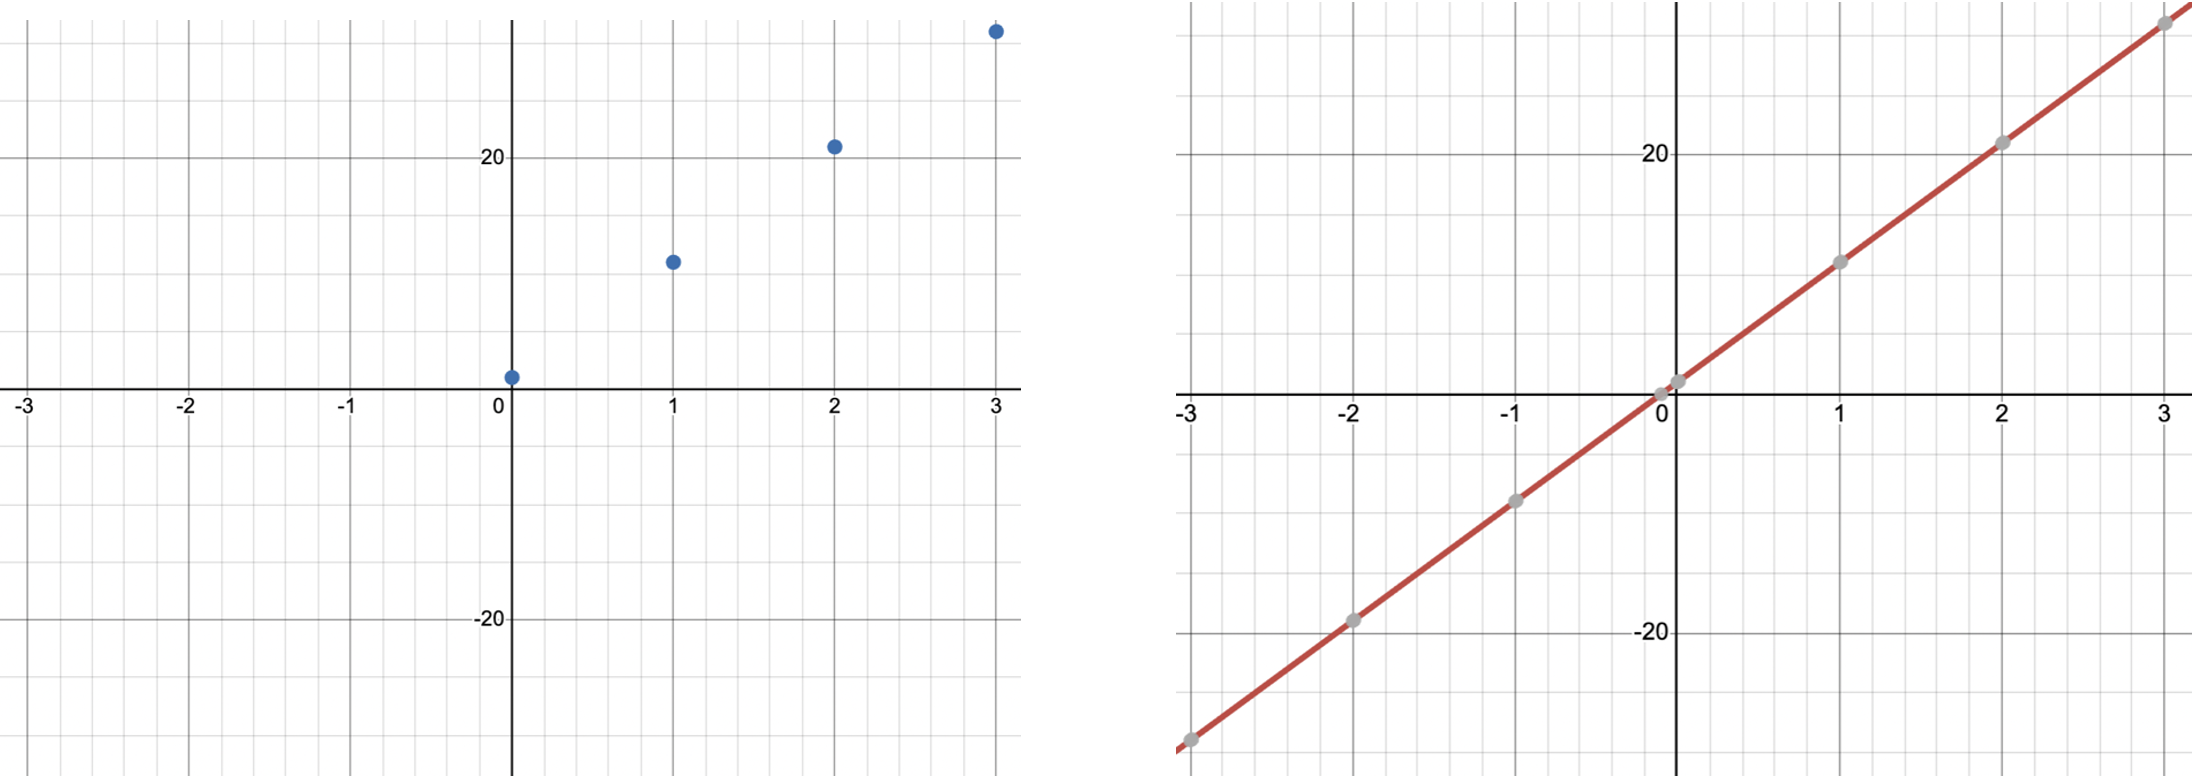
\includegraphics[scale=.35]{Images/Linear_NatvsReals_DESMOS.png}    
    \caption{Graph of the functions $f: \mathbb{N} \to \mathbb{N}$ defined by $g(n) = 10n+1$ (left) and $g: \mathbb{R} \to \mathbb{R}$ defined by $f(x) = 10x + 1$ (right).}
    \label{fig_graph_10nplus1}
\end{figure}

We used the free software {DESMOS\texttrademark} available at \url{https://www.desmos.com/} to draw the graphs in \Cref{fig_graph_10nplus1}.

When the domain and codomain are finite sets or subsets of $\mathbb{Z}$, we can draw a different representation.

\begin{defn}[Dot diagram for finite or discrete functions]
\label{defn_dot_diagram_function} 
    Consider a function $f: X \to Y$ where $X$ and $Y$ are finite sets or subsets of $\mathbb{Z}$.  The \vocab{dot diagram} for $f$ has a line of points labeled by the elements of $X$ and another line of points labeled by the elements of $Y$. If either set is infinite, then we include \ldots at one or both ends of the line of points.  For each element $x$ in the domain, we draw an arrow from the point labeled $x$ to the point labeled $f(x)$.  For example, we draw the dot diagram for the function from \Cref{exam_function_finite} in \Cref{fig_function_finite}.
            \begin{figure}[htbp]
                \centering
                %Used in \Cref{exam_function_finite}.

\begin{tikzpicture}
[scale =.5]
\GraphInit[vstyle=Welsh]
\SetUpEdge[style={->,>=triangle 45}]
\SetGraphUnit{2}
%\SetVertexNoLabel
\Vertex[LabelOut,Lpos=180,x=0,y=8]{$1$}
\Vertex[LabelOut,Lpos= 180,x=0,y=6]{$2$}
\Vertex[LabelOut,Lpos=180,x=0,y=4]{$3$}
\Vertex[LabelOut,Lpos=180,x=0,y=2]{$4$}
\Vertex[LabelOut,Lpos=180,x=0,y=0]{$5$}
\Vertex[LabelOut,Lpos=0,x=4,y=7]{$a$}
\Vertex[LabelOut,Lpos= 0,x=4,y=5]{$b$}
\Vertex[LabelOut,Lpos=0,x=4,y=3]{$c$}
\Vertex[LabelOut,Lpos=0,x=4,y=1]{$d$}
\Edges($1$, $a$)
\Edges($2$, $d$)
\Edges($3$, $a$)
\Edges($4$, $d$)
\Edges($5$, $c$)
\end{tikzpicture}
                \caption{The dot diagram of the function from \Cref{exam_function_finite}.}
                \label{fig_function_finite}
            \end{figure}
\end{defn}

Let's look at a dot diagram for a function where the domain and codomain are infinite sets.

\begin{exam}[Dot diagram for \fn{lshift}.]
\label{exam_dot_diagram_shift_left1}
    Draw the dot diagram for the function $\fn{lshift}: \mathbb{Z} \to \mathbb{Z}$ defined by $\fn{lshift}(m) = m-1$.
    \begin{soln}
        Since the domain and codomain are the set $\mathbb{Z}$ which is infinite, let's draw the points in two horizontal lines.  \Cref{fig_dot_diagram_shift_left1} shows a portion of the dot diagram, along with \ldots on each end to indicate that the pattern continues in both directions. We have drawn arrows from each integer $m$ to $\fn{lshift}(m)$, that is from $m$ to $m-1$. Many arrows are missing.  For example, the diagram does not show the arrow from -3 in the top row to -4 in the bottom row and does not show the arrow from 4 in the top row to 3 in the bottom row.
            \begin{figure}[htbp]
                \centering
                \input{Tikz/Shift_left1}
                \caption{The dot diagram of the function from \Cref{exam_dot_diagram_shift_left1}.}
                \label{fig_dot_diagram_shift_left1}
            \end{figure}
    \end{soln}
\end{exam}

Practice drawing dot diagrams.

\begin{act}[Dot diagrams of functions]
\label{act_fn_dot_diagrams}  
~
        \begin{apart}
            \item The function $s: \{1,2,3\} \to \{1,2,3\}$ is defined by $s(1) = 2$, $s(2) = 3$, and $s(3) = 1$.  Draw the dot diagram for $s$.
            \item The function $f: \mathbb{N} \to \mathbb{N}$ defined by $f(n) = 2^n$. Draw the dot diagram for $f$ as in \Cref{fig_dot_diagram_shift_left1}.  Note that the domain and codomain are $\mathbb{N}$, so there will only be \ldots on the right.          
            \item Draw the dot diagram of the constant function $h:\{1,2\} \to \{1,2\}$ defined by $h(n)=2$.  
            \item Draw the dot diagram of the identity function $i:\{1,2\} \to \{1,2\}$. 
            \item We just drew the dot diagram of two functions from $\{1,2\}$ to $\{1,2\}$.  How many other functions $k:\{1,2\} \to \{1,2\}$ are there?  Draw the dot diagram each of the other functions.
            \item How many functions $k: \{1,2\} \to \{1,2,3,4,5\}$ are there? Explain how to count. Hint: in Step 1 decide on the value of $k(1)$ and then in Step 2 decide on the value of $k(2)$.
            \item How many functions $k: \{1,2\} \to \{1,2,3,\ldots, n\}$ are there? State your answer as a conjecture involving $n$.
        \end{apart}
\end{act}

%%%%%%%%%%%%%%%%%%%%%%%%%%%%%%%%%%%%%%%%%%%

\subsection{Exercises}

%%%%%%%%%%%%%%%%%%%%%%%%

\subsubsection*{Exercises for \Cref{sub_infinite_sets_numbers} \subinfsetsnumbers}

\begin{exer}[\exerP] % Subsets of infinite sets of numbers.
\label{exer_subsets_inf_sets_numbers}
~
    \begin{exerpart}
        \item Which of the sets $\mathbb{Z}$, $\mathbb{N}$, and $\mathbb{R}^*$ have the integer -1 as an element?    
        \item Explain why $\mathbb{Z}^+$ is a subset of $\mathbb{R}^*$, but $\mathbb{N}$ is not a subset of $\mathbb{R}^*$
    \end{exerpart}
\end{exer}

\begin{exer}[\exerP] % Intervals of real numbers
\label{exer_intervals}
~
    \begin{exerpart}
        \item Write the interval $[0,2.3]$ using inequality notation.  Is 0 in the interval?  Is 2.3 in the interval? Is 5 in the interval?
        \item Write the unbounded interval $(2.3,\infty)$ using inequality notation.  Is 0 in the interval? Is 2.3 in the interval? Is 5 in the interval?
        \item Write the interval $(1,5)$ using inequality notation.  Is 0 in the interval?  Is 2.3 in the interval? Is 5 in the interval?
        \item Which integers are in the interval $(1,5)$?
        \item Write the interval $x \le 2.3$ in interval notation.  Is 0 in the interval?  Is 2.3 in the interval? Is 5 in the interval?
    \end{exerpart}
\end{exer}

\begin{exer}[\exerU] % Show real numbers are rational
\label{exer_show_rational}   
    Show that each of the following real numbers is rational by writing it in the form $\frac{a}{b}$ for some integer $a$ and some nonzero integer $b$.
        \begin{exerpart}
            \item 17.5
            \item 0.01
            \item 4
            \item $0.\overline{3}=0.333333\ldots$.          
        \end{exerpart}
\end{exer}

\begin{exer}[\exerR] % Infinite sets of numbers
\label{exer_dyk_inf_sets_numbers}
    Do you know \ldots
        \begin{exerpart}
            \item What sets the symbols $\mathbb{Z}$, $\mathbb{N}$, $\mathbb{Q}$, and $\mathbb{R}$ stand for?
            \item How the sets $S^*$ and $S^+$ are related to the set $S$?
            \item How to decide whether a number is rational?
            \item How to decide if a number is real?
            \item How to translate between inequality and interval notation?
        \end{exerpart}
\end{exer}

%%%%%%%%%%%%%%%%%%%%%%%%

\subsubsection*{Exercises for \Cref{sub_defn_function_notation} \subdefnfnnotation}

\begin{exer}[\exerP] % handshakes function   
\label{exer_hs_nplus1}
    The function $f: \mathbb{Z} \to \mathbb{Z}$ is defined by $f(n) = \frac{n(n+1)}{2}$.  Recall from \Cref{thm_hs} that $f(n)$ counts the number of handshakes in a group of $n+1$ people and so $f(n)$ is an integer.
        \begin{exerpart}
            \item Identify the domain and codomain of $f$.
            \item Evaluate $f(5)$ and $f(6)$. 
            \item Does there exist a value of $n$ such that $f(n) =6$? Explain.
            \item Does there exist a value of $n$ such that $f(n) = 5$? Explain.
            \item What is the image of the function $f$?
        \end{exerpart}
\end{exer}

\begin{exer}[\exerU] % alternating factorial]
\label{exer_alt_factorial}
    Consider the function $g: \mathbb{N} \to \mathbb{Z}$ defined by $g(n) = (-1)^nn!$ where, as usual $n!$ denotes the factorial (\Cref{defn_factorial}).
        \begin{exerpart}
            \item Identify the domain and codomain of $g$.
            \item Evaluate $g(4)$ and $g(5)$.  
            \item Could we have said that the codomain of $g$ is $\mathbb{N}$?  Explain.
            \item Since 0 is a natural number, $g(0)$ is defined.  Evaluate $g(0)$.
        \end{exerpart}
\end{exer}

\begin{exer}[\exerU] % Mod 10 function
\label{exer_fn_modn}  
    Recall that $a \fn{ mod } n$ is the remainder when $a$ is divided by n, as introduced in \Cref{defn_quo_rem_div_mod}.  
        \begin{apart}
            \item Consider the function $t: \mathbb{Z} \to \mathbb{Z}$ defined by $t(a) = a \fn{ mod } 3$.  Evaluate $t(5)$, $t(6)$, and $t(7)$.  What is the image of $t$?
            \item Consider the function $f: \mathbb{Z} \to \mathbb{Z}$ defined by $f(a) = a \fn{ mod } 4$.  Evaluate $f(5)$, $f(6)$, and $f(7)$.  What is the image of $f$? Be careful.
            \item Fix an integer $n \ge 2$ and consider the function $h: \mathbb{Z} \to \mathbb{Z}$ defined by $g(a) = a \fn{ mod } n$.  What is the image of $h$? 
        \end{apart}
\end{exer}

\begin{exer}[\exerU] %n choose 3 function
\label{exer_fn_nchoose3}
    Recall that $\binom{n}{k}$ is the number of ways to choose a subset of $k$ objects from a set of $n$ objects, as defined in \Cref{defn_binomial_coeff}. Consider the function    
    $\fn{choosethree}: \mathbb{N} \to \mathbb{Z}$ defined by $\fn{choosethree}(n) = \binom{n+3}{3}.$
        \begin{exerpart}
            \item Identify the domain and codomain of \fn{choosethree}.
            \item Evaluate $\fn{choosethree}(0)$, $\fn{choosethree}{1}$, and
            $\fn{choosethree}{2}$.
        \end{exerpart}
\end{exer}

\begin{exer} [\exerU] % function is gcd with 15
\label{exer_fn_gcd15}
    Recall that $\fn{gcd}(a,b)$ is the greatest common divisor of $a$ and $b$, as defined in \Cref{defn_gcd}. Consider the function $f: \mathbb{N} \to \mathbb{N}$ defined by $f(n) = \fn{gcd}(n,15)$.  
        \begin{exerpart}
            \item Evaluate $f(24)$, $f(10)$, and $f(7)$.
            \item Give an example of three different integers with $f(n) = 1$.
            \item Describe the image of $f$.
        \end{exerpart}
\end{exer}

\begin{exer}[\exerU] % Function counterexamples
\label{exer_fn_cex}
    Each of the following statements is false.  Find a counterexample.
        \begin{exerpart}
            \item Every function $f: \mathbb{Z} \to \mathbb{Z}$ has $f(0)=0$.
            \item The function $f: \mathbb{Z} \to \mathbb{Z}$ defined by $f(n)=n+3$ has no value of $n$ for which $f(n) = 0$. 
        \end{exerpart}          
\end{exer}

\begin{exer} [\exerU] % True or false function definition
\label{exer_TorF_no_fn}
    Decide if each statement is true or false.  If true, briefly explain why.  If false, give a counterexample.
    \begin{exerpart}
        \item \label{part_no_fn_true} No function $f$ has $f(0)=1$ and $f(0)=-1$. 
        \item \label{part_no_fn_false} No function $f$ has $f(1)=0$ and $f(-1)=0$. 
    \end{exerpart}    
\end{exer}

\begin{exer}[\exerU] % Fixed Points]
\label{exer_fixed_points_RZ}
    \Cref{defn_constant_identity_fixed_points} defines a fixed point of a function.  Find a fixed point of each function.
        \begin{exerpart}
            \item The function $q: \mathbb{R} \to \mathbb{R}$ is defined by $q(x) = 1-x$. 
            \item The constant function $c: \mathbb{Z} \to \mathbb{Z}$ is defined by $c(n) = 3$.  
            \item The function $f: \mathbb{Z} \to \mathbb{Z}$ is defined by $f(a) = a \fn{ mod } 4$ from \Cref{exer_fn_modn}.
        \end{exerpart} 
\end{exer}

\begin{exer}[\exerR] % function notation and vocab
\label{exer_dyk_fn_vocab}
    Do you know \ldots
        \begin{exerpart}
            \item What the three parts of the definition of a function are? Hint: two are sets.
            \item What the domain, codomain, and image of a function mean in terms of input and output values?
            \item How to identify the domain and codomain of a function from $f: X \to Y$ notation?
            \item How to find the image of a function?
            \item How to pronounce ``$f(x)$'' when $f$ is a function?
            \item Why we make a distinction between $f$ and $f(x)$?
            \item How to evaluate a function?
            \item What the difference is between $f(2)$ and $f(x)=2$?
            \item How to evaluate a constant function?
            \item What the rule for the identity function is?
            \item What a fixed point of a function is?
        \end{exerpart}
\end{exer}

\begin{exer}[\exerE] % prime generating function]
\label{exer_prime_quadratic}
    Consider the function $q: \mathbb{N} \to \mathbb{N}$ defined by $q(n) = n^2+n+41$.
        \begin{exerpart}
            \item  Check that $q(0)$, $q(1)$, $q(2)$, $q(3)$, $q(4)$, $q(5)$, $q(6)$, and $q(7)$ are each prime.  You may consult the list we created in \Cref{exam_sieve}.
            %\item Use \Cref{thm_show_is_prime} to show how to check by hand that $q(8)$ is prime.  Hint: You may use that $2 \mid 112$, $3 \mid 111$, $5 \mid 100$, $7 \mid 112$, and $\sqrt{113} < 11$.  %We did a similar process \Cref{exer_101_110_prime} in \Cref{sec_primes}.
            \item Find a positive integer $n$ such that $q(n)$ is composite.  Hint: Note that $q(n) = n(n+1)+41$.  Can you see a value of $n$ where $n$ or $(n+1)$ might factor out? You may use computational technology, but do not just look up the answer.
        \end{exerpart}
\end{exer}

\begin{exer}[\exerE] % consecutive ratios]
\label{exer_consecutive_ratios}
    The function $f: \mathbb{Z}^+ \to \mathbb{Q}$ is defined by $f(n) = \frac{n+1}{n}$.
        \begin{exerpart}
            \item Identify the domain and codomain of the function $f$.
            \item Evaluate $f(1)$, $f(2)$, and $f(4)$.
            \item What happens if you try to use the rule for $f$ to evaluate $f(0)$?  Why should we not be concerned about what happens?
            \item Evaluate $f(10)$, $f(100)$, and $f(\text{1,000})$.  Write your answers in decimal format.  
            \item Make a conjecture about the image of $f$.  Write your answer as an inequality.
        \end{exerpart}
\end{exer}

\begin{exer}[\exerE] % why fraction is integer]
\label{exer_consec_prod_even_fn}
    Prove that the fraction $\frac{n(n+1)}{2}$ is always an integer.  Hint: consider cases.  This proof justifies that the function $f: \mathbb{Z} \to \mathbb{Z}$ defined by $f(n) = \frac{n(n+1)}{2}$ from \Cref{exer_hs_nplus1} always produces output values in the codomain $\mathbb{Z}$.
\end{exer}

\begin{exer}[\exerE] % functions defined on $\mathbb{Z}_n$]
\label{exer_functions_on_Zn_vocab}
    Recall that $a \fn{ mod } 10$ is the remainder when $a$ is divided by 10, as introduced in \Cref{defn_quo_rem_div_mod}.  In \Cref{sec_mod_arith}, we introduced the set $$\mathbb{Z}_{10}= \{0,1,2,3,4,5,6,7,8,9\}$$
    where addition was defined by $a \oplus b = a + b \fn{ mod } 10$ and multiplication was defined by $a \otimes b = ab \fn{ mod } 10$.
    \begin{exerpart}
        \item Consider the function $g: \mathbb{Z}_{10} \to \mathbb{Z}_{10}$ defined by $g(a) = 3 \oplus a$.  What are the domain and codomain of $g$?  Evaluate $g(4)$.  Give an example of an element $a$ of $\mathbb{Z}_{10}$ such that $g(a) =1$.
        \item Consider the function $h: \mathbb{Z}_{10} \to \mathbb{Z}_{10}$ defined by $h(a) = 3 \otimes a$.  What are the domain and codomain of $h$?  Evaluate $h(4)$.  Give an example of an element $a$ of $\mathbb{Z}_{10}$ such that $h(a) =1$.
    \end{exerpart}
\end{exer}

\begin{exer} [\exerE]% Definition of increasing function
\label{exer_defn_increasing}
    Consider a function $f: X \to Y$ where $X$ and $Y$ are subsets of $\mathbb{R}$.  The function $f$ is \vocab{increasing} if for every number $a$ and $b$, if $a < b$, then $f(a) < f(b)$.
        \begin{exerpart}
            \item Use \Cref{pff_if_then_direct} to prove that the function $f: \mathbb{Z} \to \mathbb{Z}$ defined by $f(n) = 3n$ is increasing.
            \item Give a counterexample to show that the function $g: \mathbb{R} \to \mathbb{R}$ defined by $g(x) = x^2$ is not increasing.
        \end{exerpart}
\end{exer}

%%%%%%%%%%%%%%%%%%%%%%%%

\subsubsection*{Exercises for \Cref{sub_piecewise} \subpiecewise}

\begin{exer}[\exerP] % evaluate Collatz function]
\label{exer_evaluate_collatz}  
    The Collatz function $c: \mathbb{Z} \to \mathbb{Z}$ defined by 
    $$c(n) =  \left\{ 
    \begin{array} {cl} 
    \frac{n}{2} & \text{if } n \text{ is even} \\ 
    3n+1 & \text{if } n \text{ is odd} \\  
    \end{array} 
    \right.$$
        \begin{exerpart}
            \item Evaluate $c(3)$ and $c(4)$.          
            \item How many values of $n$ have $c(n) = 10$?  Explain.
            \item How many values of $n$ have $c(n) = 11$? Explain.    
        \end{exerpart}
\end{exer}

\begin{exer}[\exerP] % absolute value]
\label{exer_absolute_value}
    The function $\fn{abs}: \mathbb{Z} \to \mathbb{Z}$ is defined by 
    $$\fn{abs}(n)=
    \left\{
        \begin{array}{rl}
            n & \text{if } n \text{ is non-negative} \\
            -n & \text{if } n \text{ is negative}
        \end{array}
    \right.$$
        \begin{exerpart}
            \item Evaluate $\fn{abs}(4)$, $\fn{abs}(0)$, and $\fn{abs}(-4)$.
            \item Explain why $\fn{abs}(n)$ is always non-negative.
            \item Identify the domain, codomain, and image of $\fn{abs}$.
        \end{exerpart}
        Note: $\fn{abs}(n)$ is often denoted $|n|$.  These absolute value symbols ($|$) are at the same priority in the order of operations (\Cref{defn_integer_algebra_order_operations}) as parentheses.
\end{exer}

\begin{exer}[\exerR] % piecewise-defined functions
\label{exer_dyk_fn_piecewise}
    Do you know \ldots
        \begin{exerpart}
            \item How to evaluate a piecewise-defined function? 
            \item How to find the image of a piecewise-defined function?
        \end{exerpart}
\end{exer}

\begin{exer}[\exerE] % Collatz conjecture]
\label{exer_collatz_conjecture}
    In \Cref{exer_evaluate_collatz} we saw the Collatz function $c: \mathbb{Z} \to \mathbb{Z}$ defined by 
    $$c(n) =  \left\{ 
    \begin{array} {cl} 
    \frac{n}{2} & \text{if } n \text{ is even} \\ 
    3n+1 & \text{if } n \text{ is odd} \\  
    \end{array} 
    \right..$$  
    In this exercise, we are going \vocab{iterate} the function $c$, meaning we complete $c(n)$, then evaluate $c$ at the answer to get $c(c(n))$, then evaluate $c$ at the answer to get $c(c(c(n)))$, and so on.  
        \begin{exerpart}
            \item  Starting with $n=6$, iterate the function $c$.  This means evaluate $c(6)$, then $c(c(6))$, then $c(c(c(6)))$, and so on.  You may stop when the pattern becomes obvious.  Write down the list of values you get starting with 6.
            \item Repeat for $n=7$.
            \item What do you notice?  State your answer as a conjecture.  This conjecture is known as the \vocab{Collatz conjecture}. 
        \end{exerpart}
    You may read more about the Collatz conjecture online, but wait until after you finished the parts of this exercise so you don't spoil the surprise.
\end{exer}

\begin{exer}[\exerE] % Prove 8 is not in the image
\label{exer_8isnotinimage}
    Consider the piecewise defined function 
        $$p(n) = \left\{ 
        \begin{array}{cc} 
            n+1 & \text{ if $n$ is even} \\
            2n & \text{ if $n$ is odd} 
        \end{array}
        \right.$$ 
    Write a formal proof that $p(n) \neq 8$ for all integers $n$.  Hints: Use a proof by contradiction (\Cref{pff_contradiction}).  Within that proof, use proof by case (\Cref{pff_cases}).  See \Cref{exam_piecewise_defined_function} (\ref{part_8notinimage}) for more detail.
\end{exer}

%%%%%%%%%%%%%%%%%%%%%%%%

\subsubsection*{Exercises for \Cref{sub_fn_dot_graph} \subfndotgraphs}

\begin{exer}[\exerP] % domain, codomain, and dot diagrams of finite functions]
\label{exer_domain_codomain_finite} 
    Identify the domain and codomain for each finite function and draw its dot diagram.
        \begin{exerpart}            
            \item \label{part_first_dot_finite} $f: \{1, 2, 3, 4\} \to \{a, b, c\}$ defined by $f(1) = a, f(2) = b, f(3) = a, f(4) = c$
            \item $g: \{1, 2, 3, 4\} \to \{a, b, c, d\}$ defined by $g(1) = a, g(2) = b, g(3) = a, g(4) = c$
            \item \label{part_third_dot_finite} $h: \{1, 2, 3, 4\} \to \{1,2,3,4\}$ defined by $h(1) = 2, h(2) = 3, h(3) = 4, h(4) = 1$
            \item $k: \{1, 2, 3, 4\} \to \{1,2,3,4\}$ defined by $k(1) = 3, k(2) = 3, k(3) = 3, k(4) =3$
        \end{exerpart}  
\end{exer}

\begin{exer}[\exerP] % $n \mapsto 3n$]
\label{exer_nmapsto3n}
    The function $g: \mathbb{Z} \to \mathbb{Z}$ is defined by $g(n) = 3n$.
        \begin{exerpart}
            \item Evaluate $g(6)$ and $g(1)$. 
            \item Does there exist a value of $n$ such that  $g(n)=6$? Explain.
            \item Does there exist a value of $n$ such that $g(n)=1$? Explain.
            \item What is the image of the function $g$?
            \item Draw the dot diagram of $g$ including $n=-3,-2,-1,0,1,2,3$.
        \end{exerpart}
\end{exer}

\begin{exer}[\exerP] % $x \mapsto 1-x$]
\label{exer_1minusx}
    Consider the function $g: \mathbb{R} \to \mathbb{R}$ defined by $g(x) = 1-x$.
        \begin{exerpart}
            \item Identify the domain of $g$ and the codomain of $g$.
            \item Evaluate $g(0)$, $g(0.5)$, $g(2)$, and $g(-2)$.
            \item Find a real number $x$ with $g(x) = 2$.  How many real numbers $x$ have $g(x) = 2$?
            \item Draw the graph of $g$ on the $xy$-plane by hand.
            \item For what values of $x$ is $g(x) \ge 0$.  Answer using an inequality.% and also using interval notation.
        \end{exerpart}    
\end{exer}

\begin{exer}[\exerU] % dot diagram number-theoretic functions
\label{exer_fn_numbthy_dotdiagram}
    Pay careful attention to the domain and codomain when drawing dot diagrams.
        \begin{exerpart}
            \item Draw the dot diagram for the function $t: \mathbb{Z} \to \mathbb{Z}$ defined by $t(a) = a \fn{ mod } 3$ from \Cref{exer_fn_modn}.
            \item Draw the dot diagram for the function $\fn{choosethree}: \mathbb{N} \to \mathbb{Z}$ defined by $\fn{choosethree}(n) = \binom{n+3}{3}$ from \Cref{exer_fn_nchoose3}.
            \item Draw the dot diagram for the function  $f: \mathbb{N} \to \mathbb{N}$ defined by $f(n) = \fn{gcd}(n,15)$ from \Cref{exer_fn_gcd15}.
        \end{exerpart}
\end{exer}

\begin{exer}[\exerU] % graphing identity functions]
\label{exer_graphing_identity_function}     
    We defined the identity function in \Cref{defn_constant_identity_fixed_points}.
        \begin{exerpart}
            \item Draw the dot diagram of the identity function $i:\{1,2,3,4\} \to \{1,2,3,4\}$.
            \item Draw the dot diagram of the identity function $i: \mathbb{Z} \to \mathbb{Z}$.
            \item Draw the graph on the $xy$-plane of the identity function $i: \mathbb{R} \to \mathbb{R}$.
            \item Draw the graph on the $xy$-plane of the identity function $i: \mathbb{Z} \to \mathbb{Z}$.
    \end{exerpart}
\end{exer}

\begin{exer}[\exerU] % graphing constant functions]
\label{exer_graphing_constant}  
We defined a constant function in \Cref{defn_constant_identity_fixed_points}.
    \begin{exerpart}
        \item Draw the dot diagram of the constant function $c:\{1,2,3,4\} \to \{1,2,3,4\}$ defined by $c(n)=2$.
        \item Draw the dot diagram of the constant function $c:\mathbb{Z} \to \mathbb{Z}$ defined by $c(n)=2$.
        \item Draw the graph on the $xy$-plane of the constant function $c: \mathbb{R} \to \mathbb{R}$ defined by $c(x)=2$.
        \item Draw the graph on the $xy$-plane of the constant function $c: \mathbb{Z} \to \mathbb{Z}$ defined by $c(x)=2$.
    \end{exerpart}
\end{exer}

\begin{exer}[\exerR] % dot diagrams and graphs of functions
\label{exer_dyk_fn_dot_graphs}
    Do you know \ldots
        \begin{exerpart}
            \item How to draw the dot diagram for a function when the domain and codomain are finite?
            \item How to draw the dot diagram for a function when the domain and codomain are (possibly infinite) subsets of $\mathbb{Z}$.
            \item How to draw the graph of a function when the domain and codomain are subsets of $\mathbb{R}$?  For any complicated rule, you are welcome to use DESMOS\texttrademark.
            \item How are $x$ and $y$ related if the point $(x,y)$ is on the graph of the function $f$?
            \item Why some graphs of functions in the $xy$-plane consist of separate points while other graphs have continuous lines or curves?  
        \end{exerpart}
\end{exer}

\begin{exer}[\exerE] % counting functions on finite set]
\label{exer_count_functions_finite}
    The first three parts of this exercise duplicate our work in \Cref{act_fn_dot_diagrams}.  Hint:  A question beginning ``how many'' asks you to count.  For example, you can use that steps multiply (\Cref{thm_steps_multiply}).
    \begin{exerpart}
        \item How many functions $f:\{1,2\} \to \{1,2\}$ are there? 
        \item How many functions $f:\{1,2\} \to \{1,2,3\}$ are there? Explain how to count using steps.
        \item How many functions $f:\{1,2\} \to \{1,2,3, \ldots n\}$ are there? State your answer as a conjecture involving a function of $n$.         
        \item How many functions $f:\{1,2,3\} \to \{1,2\}$ are there? Explain how to count using steps.
        \item How many functions $f:\{1,2,3, \ldots n\} \to \{1,2\}$ are there? State your answer as a conjecture involving a function of $n$. 
    \end{exerpart}     
\end{exer}

\begin{exer} [\exerE] % graphing lines
\label{exer_desmos_lines}
    In each part of this exercise, use {DESMOS\texttrademark} to graph the functions $y =f(x)$ on the same set of axes for $-5 \le x \le 5$ and $-15 \le x \le 15$.  Some properties that could be similar or different:  is/is not a line, having the same/different slope (rise over run), having the same/different $y$-intercept (point where the graph crosses the $y$-axis), being increasing (uphill as move left to right)/decreasing (downhill as move left to right).
    \begin{exerpart}
        \item Compare the graphs of $y=x$ and $y = -x$ by saying what is similar and different. 
        \item Compare the graphs $y = x+1$ and $y = 1-x$ by saying what is similar and different. 
        \item Compare the graphs of $y=x$, $y=2x$, and $y=3x$ by saying what is similar and different.      
        \item Compare the graphs of $y = x+1$, $y = x+2$, and $y = x+3$ by saying what is similar and different. 
        \item Compare the graphs of $y=x+1$ and $y = x^2+1$ by saying what is similar and different. 
    \end{exerpart}
\end{exer}

% \begin{exer}[\exerE] % Graph Piecewise-Defined Function on Real Numbers]
% \label{exer_graph_piecewise_real_function}  
%     Consider the function $f: \mathbb{R} \to \mathbb{R}$ defined by 
%     $$f(x) = \left\{ \begin{array} {cl} x-3 & \quad \text{if } x > 0 \\ 0 & \quad \text{if } x=0 \\ x+3 & \quad\text{if } x <0 \\ \end{array} \right.$$ on the $xy$-plane.
%         \begin{exerpart}
%             \item Evaluate $f(2)$, $f(0)$, and $f(1)$.
%             \item Draw the graph of $f$ on the usual $xy$-plane by hand.  At the points where the case changes, draw a closed point (like a vertex of graph that is  colored black) to indicate that the point is on the graph and an open point (like a vertex of a graph that is  colored white) to indicate that the endpoint of the line is not included.
%         \end{exerpart}
% \end{exer}

%%%%%%%%%%%%%%%%%%%%%%%%%%%
\subsection{\answers}
%%%%%%%%%%%%%%%%%%%%%%%%%%%

%%%%%%%%%%%%%%%%%
\subsubsection{\answers for \Cref{sub_infinite_sets_numbers} \subinfsetsnumbers}

\subsubsection*{\Cref{exer_subsets_inf_sets_numbers} \answers}
\begin{apart}
    \item Hint: two of the sets contain -1.
    \item Hint: 0 in $\mathbb{N}$
\end{apart}

\subsubsection*{\Cref{exer_intervals} \answers}
\begin{apart}
    \item $0 \le x \le 2.3$,
    yes, yes, no.
    \item $x > 2.3$, no, no, yes.
    \item Hint: answer should involve $<$.
    \item Hint: three integers.
    \item Hint: the answer involves $-\infty$.
\end{apart}

%%%%%%%%%%%%%%%%%%
\subsubsection{\answers for \Cref{sub_defn_function_notation} \subdefnfnnotation}

\subsubsection*{\Cref{exer_alt_factorial} \answers}
\begin{apart}
    \item $\mathbb{N}$, $\mathbb{Z}$
    \item -24, 120 (Show work.)
    \item Hint: no
    \item Hint: $(-1)^0=1$ and $0!=1$.
\end{apart}

\subsubsection*{\Cref{exer_fn_modn} \answers}
\begin{apart}
    \item 2, 0, 1, $\{0,1,2\}$
    \item Hint: evaluate $f(8)$ too
    \item Hint: what are the possible values of $a \fn{ mod } n$?
\end{apart}

\subsubsection*{\Cref{exer_fn_nchoose3} \answers}
\begin{apart}
    \item $\mathbb{N}$, $\mathbb{Z}$
    \item Hint: $\binom{5}{3}=10$
\end{apart}

\subsubsection*{\Cref{exer_fn_gcd15} \answers}
\begin{apart}
    \item Hint: The answers in some order are 1, 3, 5.
    \item Hint: Make sure none of your examples are divisible by three or divisible by five
    \item Hint: What are the divisors of 15?
\end{apart}

\subsubsection*{\Cref{exer_functions_on_Zn_vocab} \answers}
\begin{apart}
    \item $\mathbb{Z}_{10}$, $\mathbb{Z}_{10}$, 7, 8
    \item Hint: $3 \otimes 4 = 2$
\end{apart}

\subsubsection*{\Cref{exer_defn_increasing} \answers}
\begin{apart}
    \item Hint: Your proof should begin ``\emph{Proof.} Let $a$ and $b$ be integers.  Assume $a < b$.
    \item Hint: Find real numbers $a$ and $b$ where $a < b$ but $a^2 \ge b^2$. Consider negatives.
\end{apart}

%%%%%%%%%%%%%%%%%%
\subsubsection{\answers for \Cref{sub_piecewise} \subpiecewise}

\subsubsection*{\Cref{exer_absolute_value} \answers}
\begin{apart}
    \item Hint: The answers are 0 and 4.
    \item Hint: Consider two cases.
    \item Hint: For the image consider (b). 
\end{apart}

\subsubsection*{\Cref{exer_collatz_conjecture} \answers}
\begin{apart}
    \item 3, 10, 5, 16, 8, 4, 2, 1, 4, 2, 1, 4, 2, 1, \ldots
    \item Hint: It should end the same way.
    \item It always hits 1 and then repeats.
\end{apart}

%%%%%%%%%%%%%%%%%%
\subsubsection{\answers for \Cref{sub_fn_dot_graph} \subfndotgraphs}

\subsubsection*{\Cref{exer_domain_codomain_finite} \answers}
\begin{apart}
    \item The domain is $\{1,2,3,4\}$.  The codomain is $\{a,b,c\}$, and the dot diagram is shown in \Cref{fig_answer_exer_domain_codomain_finite}.

    \begin{figure}[hbtp]
        \centering
        \begin{tikzpicture}
[scale =.35]
\GraphInit[vstyle=Welsh]
\SetUpEdge[style={->,>=triangle 45}]
\SetGraphUnit{1.6}
%\SetVertexNoLabel
\node at (2,8) {$f$};
\Vertex[LabelOut,Lpos=180,x=0,y=6]{$1$}
\Vertex[LabelOut,Lpos= 180,x=0,y=4]{$2$}
\Vertex[LabelOut,Lpos=180,x=0,y=2]{$3$}
\Vertex[LabelOut,Lpos=180,x=0,y=0]{$4$}
\Vertex[LabelOut,Lpos=0,x=4,y=6]{$a$}
\Vertex[LabelOut,Lpos= 0,x=4,y=4]{$b$}
\Vertex[LabelOut,Lpos=0,x=4,y=2]{$c$}
\Edges($1$, $a$)
\Edges($2$, $b$)
\Edges($3$, $a$)
\Edges($4$, $c$)
\end{tikzpicture}
        \caption{The dot diagram for \Cref{exer_domain_codomain_finite} (\ref{part_first_dot_finite})}
        \label{fig_answer_exer_domain_codomain_finite}
    \end{figure}

    \item Hint:  Note that $d$ is in the codomain although no arrow points into it.
    \item The domain and codomain are $\{1,2,3,4\}$. The dot diagram is shown in \Cref{fig_answer_exer_domain_codomain_finite2}.

    \begin{figure}[hbtp]
        \centering
        \begin{tikzpicture}
[scale =.35]
\GraphInit[vstyle=Welsh]
\SetUpEdge[style={->,>=triangle 45}]
\SetGraphUnit{1.6}
%\SetVertexNoLabel
\node at (2,8) {$h$};
\Vertex[LabelOut,Lpos=180,x=0,y=6]{$1$}
\Vertex[LabelOut,Lpos= 180,x=0,y=4]{$2$}
\Vertex[LabelOut,Lpos=180,x=0,y=2]{$3$}
\Vertex[LabelOut,Lpos=180,x=0,y=0]{$4$}
\Vertex[LabelOut,Lpos=0,x=4,y=6]{$ 1$}
\Vertex[LabelOut,Lpos= 0,x=4,y=4]{$ 2$}
\Vertex[LabelOut,Lpos=0,x=4,y=2]{$ 3$}
\Vertex[LabelOut,Lpos=0,x=4,y=0]{$ 4$}
\Edges($1$, $ 2$)
\Edges($2$, $ 3$)
\Edges($3$, $ 4$)
\Edges($4$, $ 1$)
\end{tikzpicture}
        \caption{The dot diagram for \Cref{exer_domain_codomain_finite} (\ref{part_third_dot_finite})}
        \label{fig_answer_exer_domain_codomain_finite2}
    \end{figure}

    \item Hint: All arrows should point to 3.
    
\end{apart}

\subsubsection*{\Cref{exer_nmapsto3n} \answers}
\begin{apart}
    \item 18, 3
    \item Hint: yes
    \item Hint: no
    \item The multiples of three.
    \item Hint: The domain and codomain are $\mathbb{Z}$ so there should be \ldots on the left and right for each row.
\end{apart}

\subsubsection*{\Cref{exer_1minusx} \answers}
\begin{apart}
    \item $\mathbb{R}$, $\mathbb{R}$
    \item Hint: The answers in some order are $-1, 0.5, 1, 3$.
    \item Hint: Solve $1-x=2$. There is one solution.
    \item Hint: The graph is a line of slope -1 with $y$-intercept 1 and $x$-intercept 1.
    \item $x \le 1$
\end{apart}

\subsubsection*{\Cref{exer_fn_numbthy_dotdiagram} \answers}
\begin{apart}
    \item Hint: All arrows should point to 0, 1, or 2.
    \item Hint: The domain is $\mathbb{N}$ so the dot diagram has $\ldots$ on the right, but the codomain is $\mathbb{Z}$ so the dot diagram has $\ldots$ on the left and right.  There should be an arrow from 0 to 1 and an arrow from 1 to 4.
    \item Hint:  The domain and codomain are $\mathbb{N}$ so the dot diagram has $\ldots$ on the right.  Every arrow points to 1, 3, 5, or 15.
\end{apart}

\subsubsection*{\Cref{exer_graphing_identity_function} \answers}
\begin{apart}
    \item Hint: All arrows should point horizontally.
    \item Hint: All arrows should point vertically.
    \item Hint: The graph is the line $y=x$.
    \item Hint: The graph consists of isolated points on the line $y=x$.
\end{apart}

\subsubsection*{\Cref{exer_graphing_constant} \answers}
\begin{apart}
    \item Hint: All arrows should point into 2.
    \item Hint: All arrows should point into 2.
    \item Hint: The graph is a horizontal line.
    \item Hint: The graph consists of isolated dots along that horizontal line. 
\end{apart}





